\documentclass[12pt, a4paper]{article}
\usepackage[utf8]{inputenc}
\usepackage[T2A]{fontenc}
\usepackage[russian]{babel}
\usepackage[top=2cm, bottom=2cm, left=2.5cm, right=1.5cm]{geometry}
\usepackage{listings}
\usepackage{xcolor}
\usepackage{graphicx}
\usepackage{hyperref}
\usepackage{indentfirst}
\usepackage{setspace}
\usepackage{listings}
\usepackage{xcolor}
\usepackage{listingsutf8} % add this in preamble
\usepackage{minted} % put in preamble

% --- SQL listing style ---
\lstdefinestyle{sql}{
    language=SQL,
    basicstyle=\ttfamily\small,
    keywordstyle=\bfseries\color{blue!70!black},
    commentstyle=\itshape\color{gray},
    stringstyle=\color{red!60!black},
    breaklines=true,
    breakatwhitespace=true,
    frame=single,
    numbers=none,
    showstringspaces=false,
    tabsize=2,
    morekeywords={SERIAL, VARCHAR, BOOLEAN, TIMESTAMPTZ, DOMAIN, TYPE,
                  ENUM, POINT, GENERATED, ALWAYS, STORED, uint2, BEGIN,
                  COMMIT, CREATE, INSERT, INTO, VALUES, REFERENCES,
                  PRIMARY, KEY, CONSTRAINT, NOT, NULL, DEFAULT, CHECK,
                  AS, AND, INT, INT4, TIME, DATE, INDEX, ON, UNIQUE,
                  DELETE, UPDATE, CASCADE, CURRENT_DATE, TRIM, INTEGER}
}

\begin{document}

% ========== TITLE PAGE ==========
\begin{titlepage}
    \centering
    \textbf{Санкт-Петербургский Национальный Исследовательский Университет ИТМО}\\
    \textbf{Факультет Программной Инженерии и Компьютерной Техники}

    \vspace{2cm}
    
\includegraphics[width=0.4\textwidth]{ITMOLogo.png}\\[1cm]

    \vspace{3cm}
    {\Large Вариант №22685\\[0.4em]
    Лабораторная работа №1\\[0.4em]
    По дисциплине Веб-программирование \\[0.4em]
    }

    \vfill
    \begin{flushright}
        Выполнил студент:\\
        Эллити Мохамед Эмад Ахмед Авад\\[1em]
        Группы:\\ P3231 \\[1em]
        Преподаватель:\\
        Ермаков Михаил Константинович\\
        Егошин Алексей Васильевич
    \end{flushright}

    \vspace{2cm}
    Санкт-Петербург 2026 г.
\end{titlepage}

% ========== SECTION 1 ==========
\section{Разработка HTML-страницы}

В рамках лабораторной работы разработана HTML-страница для определения попадания заданной точки $(X,Y)$ в указанную область координатной плоскости при заданном значении $R$.

\subsection{Структура страницы}

Страница содержит следующие основные элементы:
\begin{itemize}
    \item заголовок с номером лабораторной работы, ФИО студента, группой и вариантом;
    \item графическое представление области на элементе \texttt{Canvas};
    \item форму для ввода координат $X$, $Y$ и значения $R$;
    \item кнопку отправки данных;
    \item таблицу с результатами предыдущих проверок;
    \item кнопку очистки истории результатов.
\end{itemize}

\subsection{Ввод и проверка данных}

Для каждого параметра используется соответствующий элемент HTML-формы. Корректность введённых значений проверяется средствами JavaScript до выполнения вычислений. При обнаружении некорректных данных выполнение проверки блокируется и пользователю выводится сообщение об ошибке.

\subsection{Определение попадания точки}

После отправки формы JavaScript получает значения $X$, $Y$ и $R$ и определяет положение точки относительно заданной области.

Область разделена на несколько частей координатной плоскости. Для каждой части используется отдельное математическое условие. Полученный результат принимает одно из двух значений: точка попала в область или точка не попала в область.

\subsection{Графическое представление}

Область и координатные оси отображаются с использованием HTML5 Canvas. Масштаб графика изменяется в зависимости от выбранного значения $R$, благодаря чему область и точка остаются корректно видимыми при разных значениях радиуса.

\subsection{Хранение результатов}

Результаты проверок сохраняются в браузере с использованием механизма \texttt{LocalStorage}. Благодаря этому история результатов сохраняется после перезагрузки страницы.

В таблице отображаются значения $X$, $Y$, $R$, результат проверки, а также дата и время выполнения запроса.

Дата и время сохраняются как единый момент времени. При отображении используется локаль \texttt{ru-RU}, поэтому время автоматически преобразуется в соответствии с часовым поясом клиентского устройства.

\subsection{Оформление страницы}

Для оформления используется CSS, размещённый непосредственно внутри HTML-документа. В работе продемонстрировано применение различных типов CSS-селекторов: селекторов идентификаторов, псевдоэлементов, дочерних и атрибутных селекторов. Также используются наследование и каскадирование CSS-свойств.

Для заголовка страницы явно задан шрифт \texttt{cursive}, его размер и цвет. Отступы и внутренние поля элементов формы задаются в пикселях.

Разработанная HTML-страница предназначена для размещения на сервере Helios и доступа через веб-браузер.

\begin{figure}[H]
\centering

\includegraphics[width=0.9\textwidth]{task.png}
\label{fig}
\end{figure}


\section*{Результат выполнения}

На рисунке~\ref{fig:result} представлен результат работы разработанного веб-приложения.

\begin{figure}[H]
    \centering
    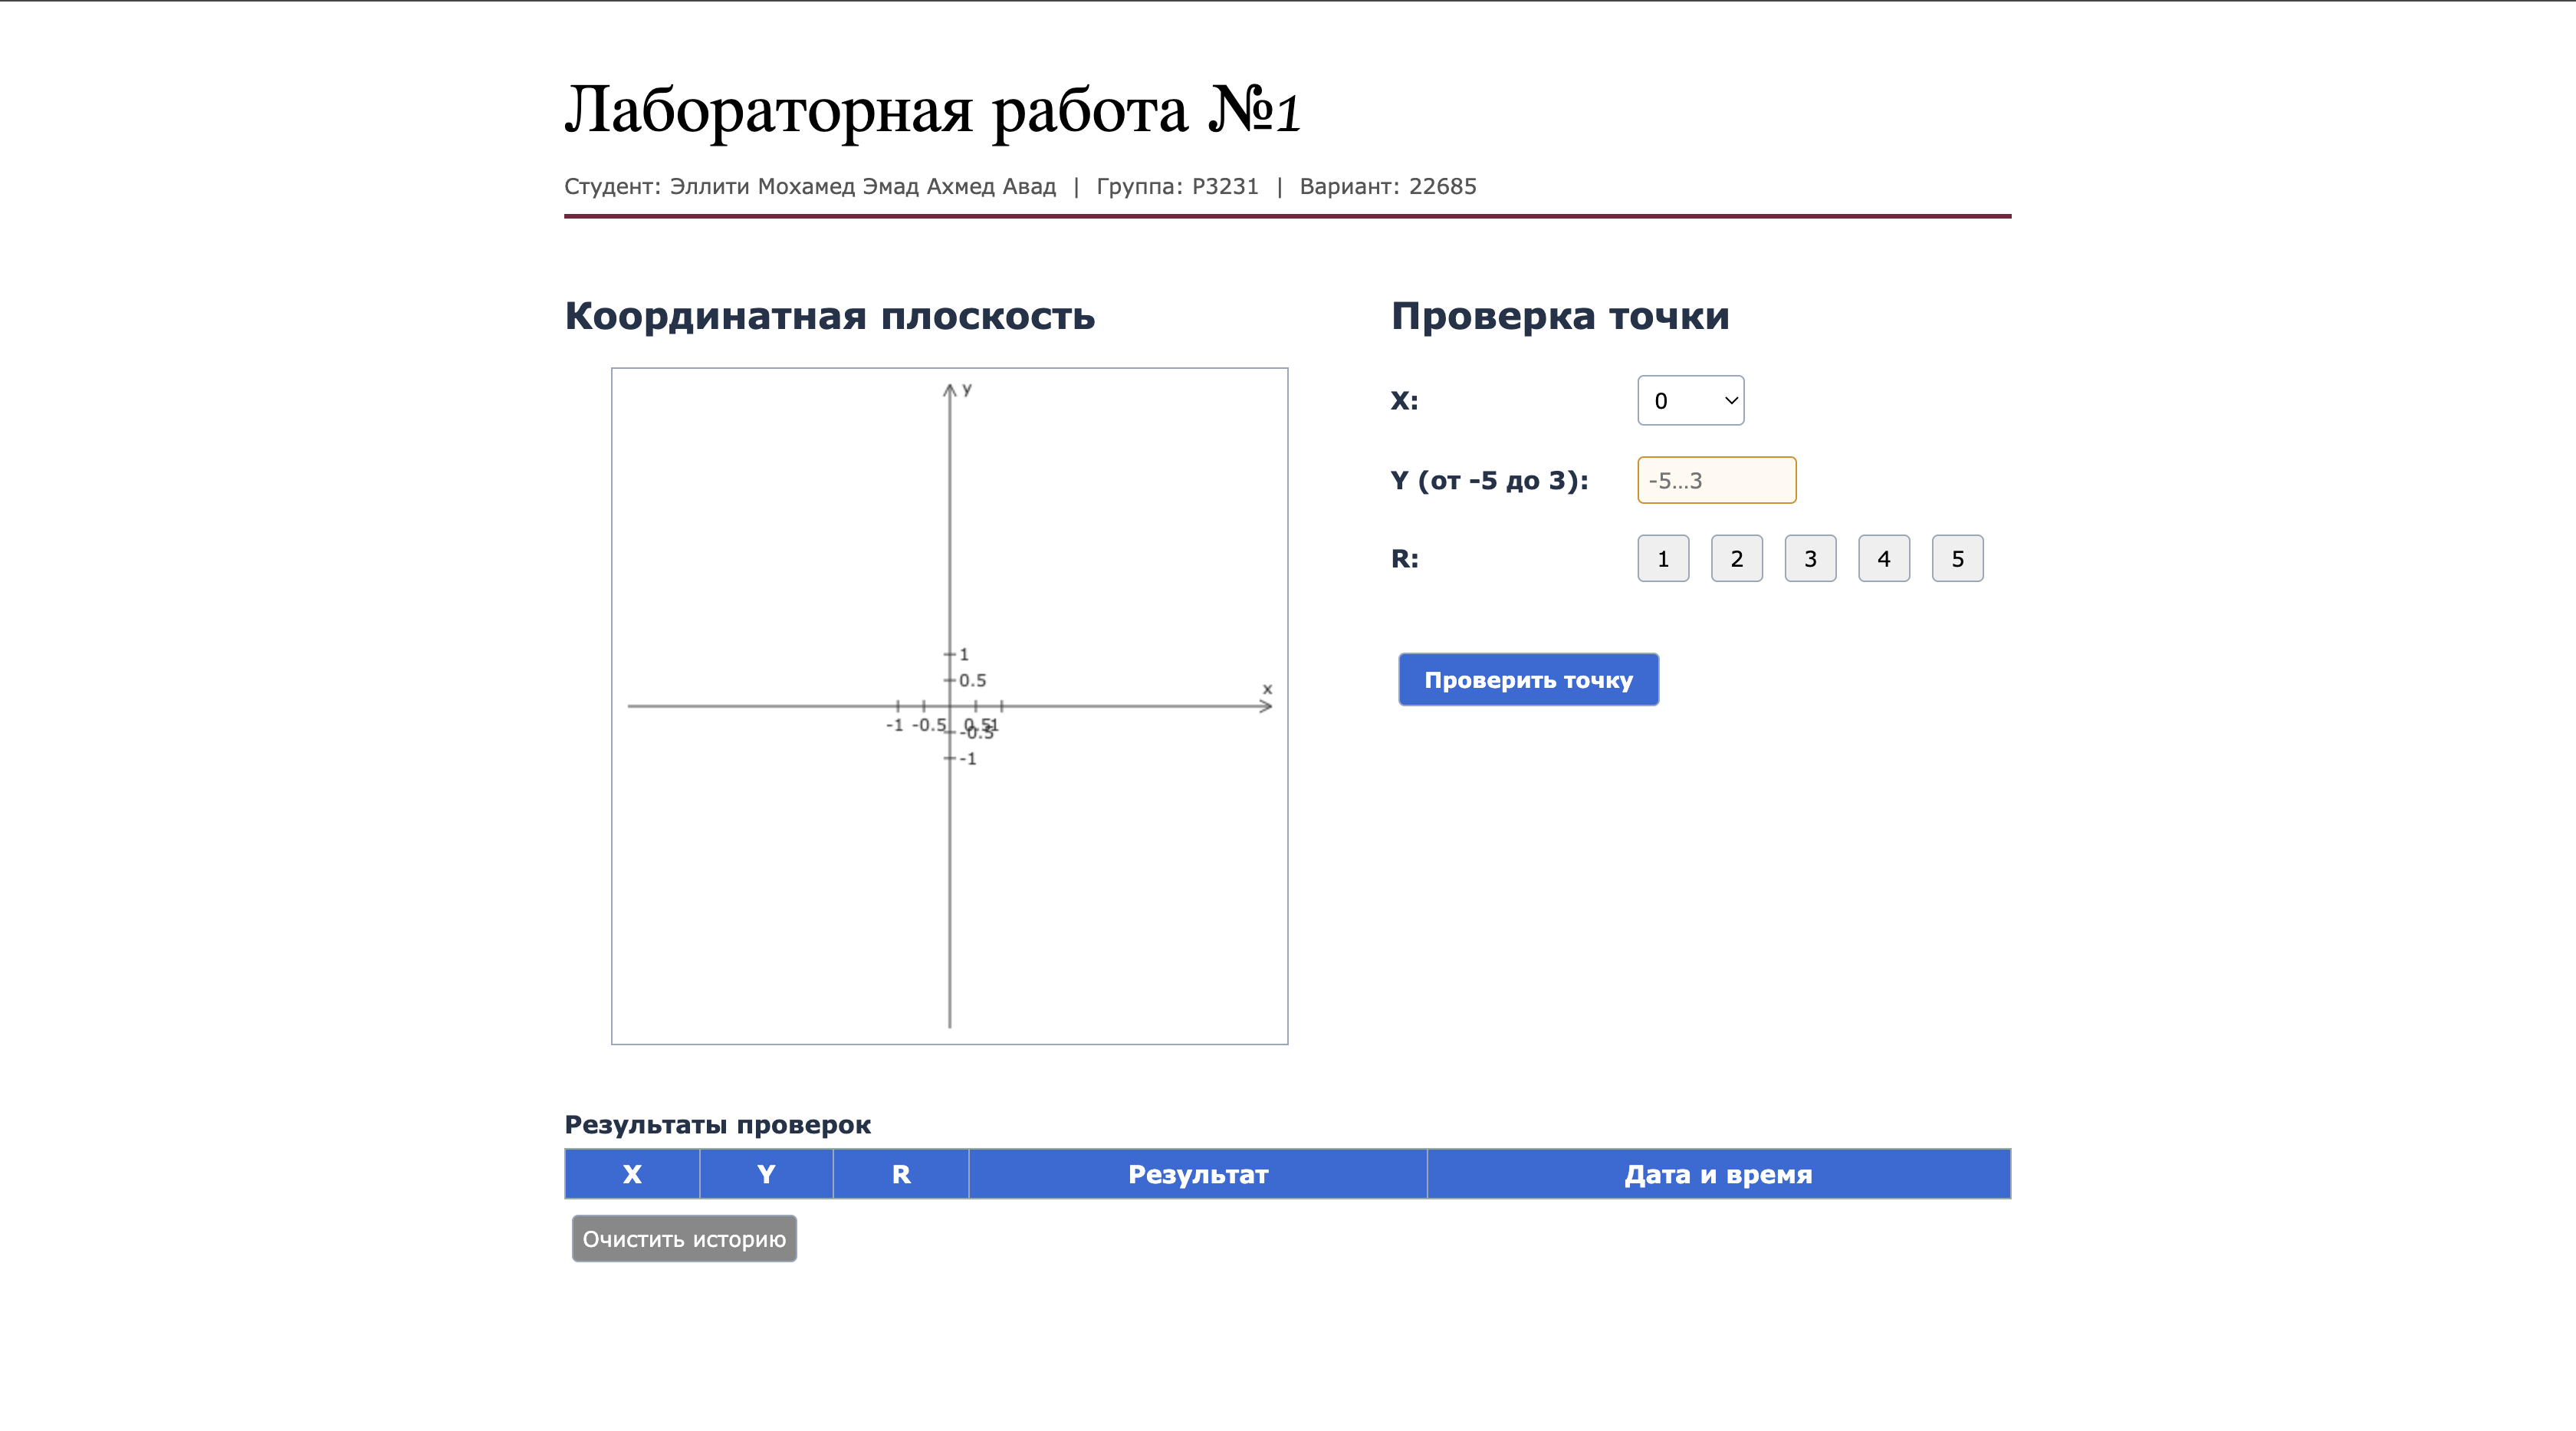
\includegraphics[width=0.9\textwidth]{result.png}
    \caption{Результат работы веб-приложения}
    \label{fig:result}
\end{figure}
% ========== SECTION 7 ==========
\section{Вывод}
В ходе лабораторной работы была разработана HTML-страница с использованием HTML, CSS и JavaScript. Реализованы проверка точки, отображение области на Canvas и сохранение результатов в LocalStorage.

Разработанное веб-приложение доступно по адресу: \\ \url{https://se.ifmo.ru/~473329/index.html}.

\end{document}